\documentclass[paper=a4, fontsize=11pt]{scrartcl} 
\usepackage[utf8]{inputenc}
\usepackage{amsmath}
\usepackage{amsfonts}
\usepackage{amssymb}
\author{Kim Thuong Ngo}


\usepackage[T1]{fontenc} 
\usepackage{fourier} 

\usepackage{lipsum} 

\usepackage{listings}
\usepackage{graphicx}
\usepackage{tabularx}

\usepackage{sectsty}
\allsectionsfont{\centering \normalfont\scshape} 

\usepackage{fancyhdr} 
\pagestyle{fancyplain} 
\fancyhead{}
\fancyfoot[L]{} 
\fancyfoot[C]{} 
\fancyfoot[R]{\thepage} 
\renewcommand{\headrulewidth}{0pt} 
\renewcommand{\footrulewidth}{0pt}
\setlength{\headheight}{13.6pt}

\numberwithin{equation}{section} 
\numberwithin{figure}{section} 
\numberwithin{table}{section}

\setlength\parindent{0pt} 

\newcommand{\horrule}[1]{\rule{\linewidth}{#1}} 

\title{	
\normalfont \normalsize 
\textsc{Algorithmen} \\ [25pt] 
\horrule{0.5pt} \\[0.4cm] 
\huge Aufgaben \\ 
\horrule{2pt} \\[0.5cm] 
}

\author{Kim Thuong Ngo} 

\date{\normalsize\today} 

%----------------------------------------------------------------------------------------

\begin{document}
\maketitle 
\newpage
\tableofcontents

%----------------------------------------------------------------------------------------
\newpage
\section{Blatt 0}
%----------------------------------------------------------------------------
\subsection{Aufgabe 1: Logarithmus}
\paragraph{a)}
Zeigen Sie: $b^{log_{b}(a)} = a$ 

$log_{b}(a) = x \Leftrightarrow b^{x} = a$

Sei $x = log_{b}(a)$ für angemessenes $x \epsilon \mathbb{R}$
$\Rightarrow b^{x} = a$
$\Rightarrow a = b^{x} = b^{log_{b}(a)}$

\paragraph{b)}
Zeigen Sie: $log_{b}(x*y) = log_{b}(x) + log_{b}(y)$

Sei $x_{1}=log_{b}(x), x_{2}=log_{b}(y)$
$\Rightarrow b^{x_{1}} = x & b^{x_{2}} = y$
$\Rightarrow x*y = b^{x_{1}}*b^{x_{2}} = b^{x_{1}+x_{2}}$
$\Rightarrow log_{b}(x*y) = x_{1} + x^{2} = log_{b}(x) + log_{b}(y)$

\paragraph{c)}
Berechnen Sie $2^{log_{4}(n)}$

$2^{log_{4}(n)}=2^{log_{2}(n^{ \dfrac{1}{2}})} = n^{\dfrac{1}{2}} = \sqrt{n}$

%----------------------------------------------------------------------------
\subsection{Aufgabe 2: Summenformel}
\paragraph{a) Kleiner Gauß}
$\sum^{n}_{i=1} i = \dfrac{1}{2} n (n+1)$

\paragraph{b)}
$\sum^{n}_{i=1} i^{3} = (\sum^{n}_{i=1} i)^{2}$

\paragraph{c)}
$\sum^{n}_{i=1} (i 2^{i}) = 2 + 2^{n+1} (n-1)$

%----------------------------------------------------------------------------
\subsection{Aufgabe 3: Ereignisraum und Ereignisse}
Lösen Sie folgende Aufgaben unter der Annahme, dass Ereignisse gleichverteilt sind.

Münze: Kopf (K), Zahl (Z)

\paragraph{a)}
Bestimmen Sie den Ereignisraum für: "Eine Münze wird drei Mal hintereinander geworfen." Betrachten Sie das Ereignis: "Es wird mindestens zwei Mal Kopf geworfen. " Wie sieht dieses Ereignis als Menge geschrieben aus? Wie ist die Wahrscheinlichkeit für dieses Ereignis?

Münze wird dreimal geworfen: $\Omega = {KKK, KKZ, KZK,ZKK,ZZK,ZKZ,KZZ,ZZZ}$
mind. zweimal Kopf: $S = {KKK,KKZ,KZK,ZKK}$
$P[S]= \dfrac{|S|}{| \Omega|} = \dfrac{4}{8} = \dfrac{1}{2}$

\paragraph{b)}
Zeigen Sie: Aus $A\cap B =\varnothing$ folgt $P[A \cup B] = P[A] + P[B]$. Was gilt, wenn $A \cap B \neq \varnothing$?

$A \cap B = \varnothing \Rightarrow P[A \cup B] = P[A] + P[B]$
$|A \cup B| = |A| + |B| - |A \cap B|$
$A \cap B = \varnothing \Rightarrow |A \cap B| = 0$
$P[A \cup B] = \dfrac{|A \cup B|}{| \Omega|} = \dfrac{|A|+|B|}{| \Omega|} = \dfrac{|A|}{| \Omega|}+ \dfrac{|B|}{| \Omega|} = P[A] + P[B]$

\paragraph{c)}
Zeigen Sie für das Gegenereignis $A^{C}= \Omega \backslash A$ eines Ergebnisses $A: P [A^{C}] = 1-P[A]$.

$A^{C} = \Omega \backslash A : P[A^{C}] = 1 - P[A]$
$ \Omega = A \cup A^{C}, A \cap A^{C} = \varnothing$
$\Rightarrow P[ \Omega] = P[A \cup A^{C}] = P[A] + P[A^{C}]$
da $P[ \Omega] = 1 \Rightarrow P[A^{C}] = 1- P[A]$

%----------------------------------------------------------------------------
\subsection{Aufgabe 4: Zufallsvariable}
Eine Zufallsvariable X ist eine Funktion $X: \Omega \rightarrow M$, wobei $\Omega$ ein Ereignisraum ist und M eine beliebige Menge. \\

Sei $\Omega = {1, ..., 10}^{2}$. Betrachten Sie die Zufallsvariable

$$X: \Omega \rightarrow \mathbb{N}, X(x,y) = x+y.$$

Wir definieren das Ereignis $[X \leq a] = {(x,y) \epsilon \Omega | X(x,y) \leq a}.$

\paragraph{a)}
Geben Sie die Menge $[X \leq 5]$ konkret an und beschreiben Sie das Ereignis in Worten.

$[X \leq 5] = {(1,1),(1,2),(1,2),(1,4),(2,1),(2,2),(2,3),(3,1),(3,2),(4,1)}$

\paragraph{b)}
Berechnen Sie $P[X \leq 5]$ unter Annahme der Gleichverteilung der Ereignisse.

$P(X \leq 5)$ bei Gleichverteilung: $|[X \leq 5]| = 10$
$| \Omega| = 10*10 = 100$
$\Rightarrow P[X \leq 5] = \dfrac{|[X \leq 5]|}{| \Omega|} = \dfrac{10}{100} = \dfrac{1}{10}$

%----------------------------------------------------------------------------
\subsection{Aufgabe 5: Erwartungswert und Varianz}
Sei $\Omega$ ein Ereignisraum. Wir definieren den Erwartungswert einer Zufallsvariable $X: \Omega \rightarrow M$ als

$$E[X] = \sum_{x \epsilon M} x * P[X=x].$$

Intuitiv beschreibt der Erwartungswert einer Zufallsvariable das Ereignis, welches im Mittel am häufigsten auftritt. Der Erwartungswert ist linear, d.h. es gilt

$$E[a+b*X] = a+b * E[X]$$

\paragraph{a)}
Berechnen Sie den Erwartungswert einer Zufallsvariable, die nur Werte 0 und 1 haben kann.

$E(X) = \sum_{x \epsilon M} x * P[X = x] = 0*P [X=0]+1*P[X=1]=P[X=1]$ 

\paragraph{b)}
Berechnen Sie den Erwartungswert eines fairen Würfels.

Erwartungswert fairer Würfel: $W={1,...,6}$
$E(X)= \sum_{x \epsilon M} x * \dfrac{1}{6} = \dfrac{1}{6} * \sum_{x \epsilon M} x = \dfrac{1}{6} * 21 = 3,5$

\paragraph{c)}
Verwenden Sie die Linearität des Erwartungswertes, um den Erwartungswert der Summe von zwei unabhängigen Würfelwürfen zu berechnen.

X: Ergebnis 1. Wurf
Y: Ergebnis 2.Wurf
$E[X+Y] = E[X]+E[Y] = 3,5 + 3,5 = 7$

\paragraph{d)}
Die Varianz einer Zufallsvariable X gibt das Mittel der quadratischen Abweichung von X zu ihrem Erwartungswert an. Formal:

$$var(X) = E[(X-E(x))^{2}].$$

Zeigen Sie mit Hilfe der Linearität des Erwartungswerts, dass folgende Gleichung gilt:

$$var(X) = E[X^{2}] - E[X]^{2}.$$

$var(x) = E [(X-E(X))^{2}]$
$= E[X^{2}] - E[X]^{2}$
$= E[X^{2}-2x*E(X)+E(X)^{2}]$
$= E[X^{2}]-E[2XE(X)]+E[E(X)^{2}]$
$= E[X^{2}]-2E(X)E(X)+E(X)^{2}$
$= E(X^{2})-2E(X)^{2}+E(X)^{2}$
$=E(X^{2})-E(X)^{2}$

%----------------------------------------------------------------------------------------
\newpage
\section{Tutorium 23.04.2018: Rekursion}

$T(0)=0$
$T(n) = 2^{n-1} + T(n-1)$
$= 2^{n-1}+2^{(n-1)-1}+T((n-1)-1)$
...
$2^{n-1}+2^{n-2}+2^{n-3}+ ... + 2^{n-i}+T(n-i)$

\underline{Vollständige Induktion}

IB: $T(n): = \sum^{i}_{k=1}2^{n-k}+T(n-i)$
IV: Behauptung gelte für beliebige feste $i \epsilon \mathbb{N}$
IA: $T(n)_{1} = \sum^{1}_{k=1} 2^{n-k}+T(n-1) = 2^{n-1}+T(n-1)$
IS: Beh: $T(n)_{i+1}= \sum^{i+1}_{k=1} 2^{n-k} + T(n-(i+1))$
$T(n):= \sum^{i}_{k=1} 2^{n-k}+ T(n-i)$
$\Rightarrow \sum^{i}_{k=1} 2^{n-i-1}+ T(n-i-1)$
$= \sum^{i}_{k=1} 2^{n-k} + 2^{n-(i+1)}+T(n-(i+1))$
$I.V.= \sum^{i+1}_{k=1} 2^{n-k} + T(n-(i+1))$
$= T(n)_{i+1}$
$\Rightarrow T(n)_{n} = \sum^{n}_{k=1} 2^{n-k} + T(n-n) $
$= \sum^{n}_{k=1} 2^{n-k}$

In welcher Laufzeitklasse liegt eine rekursive Funktion?

$T(n) = a T ( \dfrac{n}{b}) + f(n) ; a,b \geq 1; f(n), T(n) \geq 0; \varepsilon > 0$

\begin{itemize}
\item[1.Fall]
$f(n) \epsilon \mathcal{O}(n^{log_{b}(a - \varepsilon)})$ für ein $\varepsilon > 0$
$\Rightarrow T(n) \epsilon \Theta (n^{log_{b}(a)})$
\item[2.Fall]
$f(n) \epsilon \Theta(n^{log_{b}(a)}) \Rightarrow T(n) \epsilon \Theta(n^{log_{b}(a)} * log_{b}(n))$
\item[3.Fall]
$f(n) \epsilon \Omega(n^{log_{b}(a+ \varepsilon)}) \Rightarrow T(n) \epsilon \Theta (f(n))$
\end{itemize}

\begin{itemize}
\item $\mathcal{O}(n)$ Oberschranke
\item $\Omega(n)$ Unterschranke
\item $\Theta(n)$ Vereinigung beider Schranken
\end{itemize}

\subsection{Beispiele}
\underline{Mergesort}
$T(n)=2T( \dfrac{n}{2}) + n$
$a=2, b=2,f(n)=n$
$n^{log_{2}2}=n \Rightarrow 2.Fall: T(n) \epsilon \Theta(n*log_{2}n)$

\underline{binarySearch}
$T(n)=T(\dfrac{n}{2})+1$
$a=1,b=2,f(n)=1$
$1^{log_{2}1}=1 \Rightarrow2.Fall$

%----------------------------------------------------------------------------------------
\newpage
\section{Blatt 01}
%----------------------------------------------------------------------------
\subsection*{Aufgabe 1: O-Notation}
\paragraph{a)}

Aus $f_{1}(n), f_{2}(n) = \mathcal{O}(g(n))$ folgt $f_{1}(n) + f_{2}(n) = \mathcal{O}(g(n))$ und $f_{1}(n) \cdot f_{2}(n) = \mathcal{O}(g(n)^{2})$. \\

\paragraph{b)}
Aus $f(n) = \mathcal{O}(g(n))$ und $g(n) = \mathcal{O}(h(n))$ folgt $f(n) = \mathcal{O}(h(n))$. \\

\paragraph{c)}
$f(n) = \Theta (g(n))$ genau dann, wenn $g(n) = \Theta (f(n))$. \\

\paragraph{d)}
$f(n) = \mathcal{O} (g(n))$ genau dann, wenn $g(n) = \Omega (f(n))$. \\

%----------------------------------------------------------------------------
\subsection*{Aufgabe 2: Mastertheorem}
Bestimmen Sie die Komplexitätsklasse für folgende Rekursionsgleichung mit Hilfe des Mastertheorems:

\paragraph{a)}
$T(n) = T( \dfrac{n}{2}) + 1$

\begin{itemize}
\item $a = 1$
\item $b = 2$
\item $f(n) = 1$
\end{itemize}

$n^{log_{2}(1)} = n^{0} = 1$
$\Rightarrow 2. Fall$
$f(n) \in \Theta (1)$
$\Rightarrow T(n) \in \Theta(log n)$

\paragraph{b)}
$T(n) = 2T( \dfrac{n}{2}) + 1$

\begin{itemize}
\item $a = 2$
\item $b = 2$
\item $f(n) = 1$
\end{itemize}

$n^{log_{2}(2- \varepsilon)} = n^{log_{2}(2-1)} = n^{0} = 1$
$\Rightarrow 1. Fall$
$f(n) \in \Theta (1)$
$\Rightarrow T(n) \in \Theta(log n)$

\paragraph{c)}
$T(n) = 2T( \dfrac{n}{2}) + n$

\begin{itemize}
\item $a = 2$
\item $b = 2$
\item $f(n) = n$
\end{itemize}

$n^{log_{2}(2)} = n^{1} = n$
$\Rightarrow 2.Fall$
$f(n) \in \Theta (1)$
$\Rightarrow T(n) \in \Theta(log n)$

%----------------------------------------------------------------------------
\subsection*{Aufgabe 3: Rekursionen aus alten Klausuren und geometrische Summenformel}
\paragraph{a)}

Zeigen Sie, dass für folgende Rekursion $T(n) = \Theta (n^{2} log n)$ ist. 

$$T(1) = 0$$ 
$$T(n) = T(n-1) + n log n $$

\paragraph{b)}
Sei $n = ( \dfrac{8}{7})^{k}$ für ein $k \epsilon \mathbb{N}$. Folgende Rekursion ist für die Funktion T gegeben:

$$T(1)=0$$
$$T(n)= \dfrac{7}{8} T(\dfrac{7}{8} n) + \dfrac{7}{8} n$$

Finden Sie für $T(n)$ eine geschlossene Form ohne das Mastertheorem zu verwenden und beweisen Sie die Korrektheit Ihrer geschlossenen Form mit vollständiger Induktion.

\paragraph{c)}
Sei $n = (\dfrac{3}{2})^{k}$ mit $k \epsilon \mathbb{N}$. Folgende Rekursion ist für die Funktion T gegeben:

$$T(1)=0$$
$$T(n)= 2T ( \dfrac{2}{3} n) + 1$$

Finden Sie für $T(n)$ eine geschlossene Form ohne das Mastertheorem zu verwenden und beweisen Sie die Korrektheit Ihrer geschlossenen Form mit vollständiger Induktion.

\paragraph{d)}
Sei n eine Zweierpotenz, das heißt $n = 2^{k}$ für ein $k \epsilon \mathbb{N}$. Folgende Rekursion ist für die Funktion T gegeben: Für $n > 1$ gelte

$$T(n) = A(n) + B(n) ,$$ wobei
$$A(n)=A(\dfrac{n}{2}) + B( \dfrac{n}{2})$$ und
$$B(n)=B(n-1)

+2n-1.$$

Die Endwerte seien $T(1)=1$, $B(1)=1$ und $A(1)=0$. Finden Sie für $T(n)$ eine geschlossene Form ohne das Mastertheorem zu verwenden und beweisen Sie die Korrektheit Ihrer Lösung.

%----------------------------------------------------------------------------------------

\section{Ternäre Suche}
Bei der binären Suche ist der Input ein sortiertes Array $A$ und eine Zahl $x$ (die nicht notwendig im Array $A$ vorkommen muss). Dabei wird $A$ in zwei gleich große Teile $A_1$ und $A_2$ geteilt und ermittelt, in welchem der beiden Teile sich $x$ befinden müsste. Dieses Verfahren wird \emph{rekursiv} fortgesetzt. Betrachten Sie nun die \emph{ternäre Suche}, bei der $A$ statt in zwei Teile, in \emph{drei} etwa gleich große Teile $A_1$, $A_2$ und $A_3$ geteilt wird.


\paragraph{a)}
Geben Sie ein Array $A$ und ein zu suchendes Element $x$ an, so dass die binäre Suche mit weniger Vergleichen auskommt als die ternäre Suche. \\

$A:= \begin{tabular}{|c|c|c|c|c|c|c|}
\hline
0 & 1 & 2 & 3 & 4 & 5 & 6\\
\hline
\end{tabular}$ \\
ges: \textbf{3} \\

binäre Suche: \\
$\lceil \dfrac{6-0}{2} \rceil + 0 = 3.$ Position wird betrachtet \\
$\rightarrow$ \textbf{3} gefunden \\

ternäre Suche: \\
$\lceil \dfrac{6-0}{3} \rceil + 0 $ und $\lceil \dfrac{6-0}{3} \rceil + (\lceil \dfrac{6-0}{3} \rceil + 0)$, also Position 2 und 4 betrachtet \\
$\rightarrow$ \textbf{3} nicht gefunden \\
$\rightarrow$ neues Sucharray von Position 3 bis 3 \\
$\rightarrow$ Array Größe 1 \\
$\rightarrow$ \textbf{3} wird gefunden \\

Bei der binären Suche wird \textbf{3} also mit dem ersten Vergleich gefunden, bei der tertiären Suche jedoch erst nach dem drittem. 

\paragraph{b)} 
Geben Sie ein Array $A$ und ein zu suchendes Element $x$ an, so dass die ternäre Suche mit weniger Vergleichen auskommt als die binäre Suche. \\

$A:= \begin{tabular}{|c|c|c|c|c|c|c|}
\hline
0 & 1 & 2 & 3 & 4 & 5 & 6\\
\hline
\end{tabular}$ \\
ges: \textbf{2} \\

binäre Suche: \\
$\lceil \dfrac{6-0}{2} \rceil + 0 = 3.$ Position wird betrachtet \\
$\rightarrow$ Sucharray bis Position 3 betrachten: $\lceil \dfrac{3-0}{2} \rceil + 0 = \lceil 1,5 \rceil = 2$ \\
$\rightarrow$ Position 2 betrachten \\
$\rightarrow$ \textbf{2} gefunden \\
$\rightarrow$ 2 Vergleiche \\

ternäre Suche: \\
$\lceil \dfrac{6-0}{3} \rceil + 0 = \lceil 2 \rceil$ \\
$\rightarrow$ Position 2 betrachten \\
$\rightarrow$ \textbf{2} gefunden \\
$\rightarrow$ ein Vergleich \\

\paragraph{c)} 
Geben Sie Pseudocode für die ternäre Suche an. Verwenden Sie dabei Rekursion. Nummerieren Sie die Zeilen in Ihrem Pseudocode und erklären Sie detailliert jede Zeile Ihres Codes. \\

\begin{algorithm}[H]
\SetAlgoLined
\KwIn{sortiertes Array A, Integer x}
\KwOut{Integer [Postion von x in A]}
$oben \leftarrow length(1)-1$\\
$unten \leftarrow 0$\\
\textbf{while} $(oben \geq unten)$ \\
$a \leftarrow \lceil \dfrac{oben-unten}{3} \rceil$ \\
\textbf{if} ($A(a+ unten) > x$) do \\
$oben \leftarrow a+unten-1$ \\
\textbf{else if} ($A(2a+unten) < x $) do\\
$unten \leftarrow 2a+unten+1$ \\
\textbf{else if} ($A(2a+unten) > x $) do\\
$unten \leftarrow a+unten+1$ \\
$oben \leftarrow 2a+unten-1$ \\
\textbf{else if} ($A(a+unten) == x $) do\\
\Return $(a+unten)$ \\
\textbf{else} \Return -1 \\
\textbf{end} while
\end{algorithm}


\underline{Erklärung:} \\
Betrachte Array A \\
Falls $x \in A_{1}$,so prüft das der if-case in Zeile 5 \\
Falls $x \in A_{3}$,so prüft das der if-case in Zeile 7 \\
Falls $x \in A_{2}$,so prüft das der if-case in Zeile 9 \\
Falls $x=A$ oder $x=2a$, so prüfet das die if-cases in Zeile 12 und 14 \\
Falls $x \notin A_{1},A_{2},A_{3}$ und $x \neq a, x \neq 2a$ so kann x nicht im geordneten Array A existieren.

\paragraph{d)}
Analysieren Sie die Zeitkomplexität der ternären Suche. Was können Sie über die asymptotische Laufzeit der ternären Suche im Vergleich zur binären Suche sagen? \\

$T(n)=T( \dfrac{n}{3})+c$ mit $c \in {1,2,3,4,5}$ ist die passende Rekursionsgleichung, da der Suchbereich nach jedem Rekursionsschritt nur noch $\dfrac{1}{3}$ des vorherigen Suchbereiches groß ist. c ist eine Konstante (für die Vergleiche pro Rekursionsschritt) und ist immer 1,2 oder 3, außer das Element wird gefunden bzw. existiert nicht. \\
Im Mittel wird $x \approx 2$ sein. \\
Mit dem Master-Theorem: \\
$n^{log_{3}(1)} = n^{0} = 1 \in c$ \\
$\Rightarrow T(n) \in \Theta (n^{log_{3}(1)} log(n)) $ \\
$T(n) \in \Theta(log (n))$ \\
Die binäre und ternäre Suche sind also asymptotisch gleich. Es gibt also keine signifikanten Laufzeitunterschiede zur binären Suche.

\paragraph{e)}
Bei jedem Rekursionsschritt werden ein oder zwei Vergleiche benötigt, um zu entscheiden, in welchem Teil des Arrays $A$ das Element $x$ liegt. Was ist die minimale, die durchschnittliche und die maximale Anzahl an Vergleichen die benötigt wird, wenn $x$ nicht in $A$ liegt. \\

Nehme an Array A hat Größen und $x \notin A$. \\
Minimale Anzahl von Vergleiche (best case): 5 Vergleiche, falls $x \notin A_{1},A_{2},A_{3}$ und $x \neq a, x\neq 2a$ im ersten Schritt. \\
Maximale Anzahl (worst case): $\dfrac{n}{3} * 3^{n}+2 = n * 3^{n-1}+2$, falls bis Arraygröße $n=1$ aufgelöst wird und dann erst festgestellt wird $x \notin A$. \\
Durchschnittliche Anzahl (average case): $\dfrac{n*3^{n-1}+2+5}{2} = \dfrac{n}{2} *3^{n-1}+3,5$

\section{Eine Anwendung der Binären Suche}
Sei $A$ ein sortiertes Array der Größe $n$ und sei $z$ eine gegebene Zahl. Das Ziel dieser Übung ist es, folgdende Frage zu beantworten: Gibt es in $A$ zwei verschiedene Elemente $x$ und $y$, so dass $x+y=z$?

\paragraph{a)}
Es sollte nicht schwierig sein, einen Algorithmus zu finden, der diese Frage in quadratischer Zeit $\calO(n^2)$ beantwortet. Geben Sie Pseudocode für einen solchen Algorithmus an und erklären Sie warum Ihr Algorithmus die Laufzeit $\calO(n^2)$ hat. \\

\begin{algorithm}[H]
\SetAlgoLined
\KwIn{sortiertes Array A, Integer z}
\KwOut{boolean[ob $x,y \in A$ mit $x+y=z$]}
$counter \leftarrow 0$\\
$counter2 \leftarrow 0$\\
\textbf{while} $(counter2 \leq length(A)-1)$ \\
\textbf{while} $(counter \leq length(A)-1)$ \\
\textbf{if} $(A(counter)+A(counter2) == z)$ \\
\textbf{if} $(counter =! counter2)$ \\
\Return $true$ \\
\textbf{else} counter++ \\
\textbf{end} while \\
counter2++ \\
\textbf{end} while \\
\Return $false$
\end{algorithm}

Der Algorithmus hat $\mathcal{O}(z)$ Laufzeit, weil hier jede Zelle des Arrays einmal mit jeder anderen addiert und anschließendauf Größe = z verglichen wird.

\paragraph{b)}
Verwenden Sie nun die binäre Suche, um einen effizienteren Algorithmus zu finden, der die obige Frage in einer Laufzeit von $\calO(n\log n)$ beantworten kann. Geben Sie auch hier Pseudocode an und begründen Sie die Korrektheit Ihres Algorithmus. Erklären Sie, warum Ihr Algorithmus die angegebene Laufzeit hat. \\

\begin{algorithm}[H]
\SetAlgoLined
\KwIn{sortiertes Array A, Integer z}
\KwOut{}
$counter \leftarrow 0$\\
$oben \leftarrow length(A)-1$\\
$unten \leftarrow 0$ \\
\textbf{while} $(counter \leq length(A)-1)$ \\
$y=z-A(counter)$ \\
\textbf{if}$(binarySearch(y) > 0)$ \\
\Return $true$ \\
\textbf{end} while \\
\Return $false$ \\
\end{algorithm}

Da nun das Komplementärelement von y (also x mit $x+y=z$) nicht mehr in linearer Suchzeit, sondern logarithmischer Suchzeit $log(n)$ gefunden wird, falls vorhanden, benötigt dieser Algorithmus für jede Rekursion nicht mehr $\mathcal{O}(n)$ sondern $\mathcal{log(n)}$ Schritte, was bei Tests für alle n Elemente des Input Arrays zu maximal $n*log(n)$ Schritten führt, was bedeutet, dass die Laufzeit in $\mathcal{O}(n*log(n))$ liegt.

\paragraph{c)}
Es ist klar, dass ein Algorithmus für die obige Frage mindestens die Laufzeit $\Omega(n)$ benötigt. Versuchen Sie, einen Algorithmus zu finden, der obige Frage in einer Laufzeit von $\calO(n)$ beantwortet. Geben Sie Pseudocode an und begründen Sie die Laufzeit und die Korrektheit Ihres Algorithmus. \\

\begin{algorithm}[H]
\SetAlgoLined
\KwIn{sortiertes Array A, Integer z}
\KwOut{boolean[ob $x,y \in A$ mit $x+y=z$]}
$counter \leftarrow 0$\\
$oben \leftarrow length(A)-1$\\
\textbf{while} $(counter \leq length(A)-1)$ \\
$y=z-A(counter)$ \\
\textbf{if}$(binarySearch(A ,y $; ab Counter +1 Index)$ > 0)$ \\
\Return $true$ \\
\textbf{end} while \\
\Return $false$ \\
\end{algorithm}

Weil nun die Größe des binär durchsuchten Arrays in jedem Rekursionsschritt um 1 sinkt haben wir nicht mehr $log(n)$ Aufwand pro Rekursionsschritt, sondern $log(n-i)$ für das i-ten Rekursionsschritt. Das Array A(ab Counter +1) ist das Array ab der Position 5 (als untere Grenze für die binäre Suche) oder das Array ab Position 5 kopiert und als neues Array in die binarySearch mit gesuchtem y als Input gegeben. Das darf gemacht werden, weil ja die schon abgeleiteten A(Counter) sicher kein Komplementärelement haben und dementsprechend auch keines sein können und somit bei der Suche ignoriert werden.

\section{Implementierung von Suchalgorithmen}
Laden Sie die Java-Vorlage aus dem Moodle herunter und implementieren Sie die folgenden Methoden:

\begin{enumerate}
\item die Lineare Suche in \texttt{linearSearch(int[] array, int key)}. 
\item die Binäre Suche in \texttt{binarySearch(int[] array, int key)}.
\item die Interpolationssuche in \texttt{interpolationSearch(int[] array, int key)}.
\end{enumerate}
Für die Implementierung der Interpolationssuche benutzen Sie die folgende Variante aus der Vorlesung, um das jeweils nächste Element zu bestimmen:
\[ next \leftarrow \left\lceil \frac{a-S[unten-1]}{S[oben+1]-S[unten-1]} \cdot (oben-unten+1) \right\rceil + (unten-1) \]

siehe Main.java

%----------------------------------------------------------------------------------------
\section{Sortieren}
Betrachten Sie die Algorithmen \texttt{Insertionsort} und \texttt{Minimumsuche + Austausch} (Schematisch erklärt in Foliensatz 4, Seite 2).

\paragraph{a)}
Geben Sie jeweils Pseudocode für \texttt{Insertionsort} und \texttt{Minimumsuche + Austausch} an. \\

\begin{lstlisting}
Insertionsort:

Input: Array A
Output: Sortiertes Array S

n = length(A) - 1
g = 0

while(g < n) do
    ticker = g;
    x = A[g+1];
    while(A[g+1] <= A[ticker]) do
        A[ticker + 1] = A[ticker];
        if (ticker == 0) do
            brake;
        end if
        ticker --;
    end while
    A[ticker + 1] = x;
    g++;
 end while
 
 return A;

\end{lstlisting}

\begin{lstlisting}
Minimumssuche + Austausch:

Input: Array A
Output: Sortiertes Array S

n = length(A) - 1
i = 0

while (i < n) do
    min = i;
    j = i + 1;
    while(j <= n) do
        if(A[min]>A[j]) do
            min =j;
        end if
        j++;
    end while
    x = A[i];
    A[i]= A[min];
    A[min] = x;
    i++;
end while

return A;

\end{lstlisting}

\paragraph{b)}
Argumentieren Sie, dass beide Sortierverfahren korrekt sortieren. \\

Insertion-Sort:\\
Bei Insertion Sort wird von einer aufsteigenden Grenze g bis n = length(A) - 1 immer abwärts verglichen ob das Element direkt nach g (also g+1) kleiner als einer seiner Vorgänger ist, bis dieses es schließlich nicht mehr ist.\\
Dabei wird, bevor A[g+1] verglichen wird, dieses der Inhalt dieses Arrayfeldes als x gespeichert um später an die passende Position eingesetzt werden zu können und nach jedem Vergleich bei dem A[g+1] kleiner ist das betrachtete Element eine Position weiter nach rechts geschoben (weswegen A[g+1] auch gespeichert werden musste).\\
Ganz grob/kurz gesagt:\\
- Insertion Sort geht von links nach rechts durch\\
- Grenze zunächst auf erstem Element (an Position 0)\\
- Grenze steigt nach jedem Schritt um 1\\
- bei jedem Schritt wird das Element direkt nach der Grenze mit jedem Element zuvor verglichen bis es größer ist und passen eingeordnet.\\


Minimumsuche + Austausch:\\
In Zeile 12 bis 17 wird das Minimum gesucht. In Zeile 18 bis 20 wird getauscht.\\
Hierbei tickt i von 0 bis n = length(A)-1 hoch und vertauscht bei jedem Schleifendurchgang das gefundene Minimum (welches immer ab Position i linear gesucht wird) mit dem Element an der i-ten Position.\\
Sobald i = n erreicht wird, ist das letzte Element automatisch richtig sortiert und daher wird schon bei while(i kleiner n) [Zeile 9] abgebrochen und anschließend das (sortierte) Array zurückgegeben.\\

\paragraph{c)}
Geben Sie die Anzahl der Vergleiche und die Anzahl der Vertauschungen auf einer vorsortierten Eingabe der Länge $n$ an. \\

Insertion Sort:\\
Vergleiche: 1 (erstes A[0] mit zweitem A[1]) + ... + 1 (vorletztes A[n-1] mit letztem A[n]) = n - 1 Vegleiche.\\
Austausche: Theoretisch n - 1 mal, da das betrachete Element von A[g + 1] bei vor jedem g++ durch sich selbst überschrieben wird, wenn man das als Vertauschung zählt. Zählt man das "sich selbst austauschen/überschreiben" nicht, so sind es 0 Vertauschungen.\\
\\
Minimumsuche + Austausch:\\
Vergleiche: Da bei der Minimumssuche jedes Element nach Position i im Array einmal komplett durchlaufen wird: n + (n - 1) + ... + 1 = $((n+1)*n)/2$ Vergleiche.\\
Austausche: Da nach jeder Minimumssuche genau einmal (mit sich selbst vertauscht/durch sich selbst überschieben) Vertauscht wird, wird bei gesamtem Durchlauf des Arrays, wie oben theoretisch n mal getauscht. Zählt man eine Selbstüberschreibung jedoch nicht als Tausch, so sind es 0 Austausche, da die Folge bereits sortiert ist und jedes Element bereits an seinem einzufügenden Platz nach der Minimumssuche saß/sitzt.

\paragraph{d)}
Konstruieren Sie für allgemeines $n\in \mathbb N$ je ein Beispiel, auf denen die Algorithmen eine maximale Anzahl von \textit{Vergleichen} benötigt. Geben Sie diese Anzahl auch an. \\

Array mit $a_{i}>a_{i+1}$:\\
\\
Insertion Sort:\\
Weil der Reihe nach vorgegangen wird und die Eingabe von groß nach klein sortiert ist, werden für jeden Schritt i, genau i Vergleiche benötigt, um die richtige Position des Elements zu bestimmen:$\sum_{i=1}^n i = \frac{n^2+n}{2}$ Vergleiche.\\
\\
Minimumsuche + Austausch:\\
Bei der Minimumssuche muss das Array immer vollständig durchlaufen werden. Es ergibt sich also $\sum_{i=1}^n i = \frac{n^2+n}{2}$ Vergleiche.

\paragraph{e)} Konstruieren Sie für allgemeines $n\in \mathbb N$ je ein Beispiel, auf denen die Algorithmen eine maximale Anzahl von \textit{Vertauschungen} benötigt. Geben Sie diese Anzahl auch an. \\

Array mit $a_{i}>a_{i+1}$:\\
\\
Insertion Sort:\\
Weil der Reihe nach vorgegangen wird und die Eingabe von groß nach klein sortiert ist, werden für jedes g genau g Vertauschungen benötigt bis das Element sein passende Stelle gefunden hat und für jedes nächste g, das Element wieder ganz nach links geschoben wird.\\
Es ergeben sich $\sum_{i=1}^n i = \frac{n^2+n}{2}$ Vertauschungen.\\
\\
Minimumsuche + Austausch:\\
Die Anzahl der Vertauschungen liegt hier statisch bei n (außer man zählt nicht wenn ein Element mit sich selbst vertauscht wird und gerade dann wäre dies hier sicher n).

%----------------------------------------------------------------------------
\section{Heapsort}
Gegeben sei das Array $A=\langle 4,2,12,10,18,14,6,16,8 \rangle$. 

\paragraph{a)}
Bilden Sie schrittweise (Element für Element) den Min-Heap $S$ für das Array $A$. Benutzen Sie dabei die Heap-Eigenschaft: Jeder Baumknoten $u$ ist mit einem Element $S[u]$ beschriftet und es gilt: Ist $u$ Elternknoten von $v$, so ist $S[u] \leq S[v]$. Veranschaulichen und kommentieren Sie alle Schritte. \\

\begin{center}
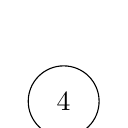
\begin{tikzpicture}[scale=0.15]
\tikzstyle{every node}+=[inner sep=0pt]
\draw [black] (37.5,-7.9) circle (3);
\draw (37.5,-7.9) node {$4$};
\end{tikzpicture}
\end{center}
Schritt 1: 1. Array-Element wird in leeren Heap eingefügt.\\

\begin{center}
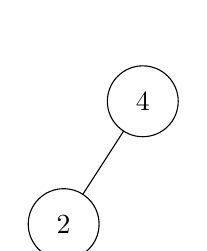
\begin{tikzpicture}[scale=0.15]
\tikzstyle{every node}+=[inner sep=0pt]
\draw [black] (37.5,-7.9) circle (3);
\draw [black] (30.8,-18.3) circle (3);
\draw (37.5,-7.9) node {$4$};
\draw (30.8,-18.3) node {$2$};
\draw [black] (35.88,-10.42) -- (32.42,-15.78);
\end{tikzpicture}
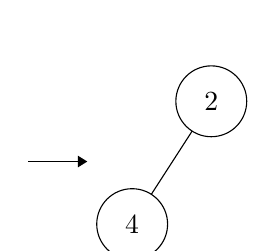
\begin{tikzpicture}[scale=0.15]
\tikzstyle{every node}+=[inner sep=0pt]
\draw [black] (22.00,-13.00) -- (27.00,-13.00);
\fill [black] (27.00,-13.00) -- (26.2,-12.5) -- (26.2,-13.5);
\draw [black] (37.5,-7.9) circle (3);
\draw [black] (30.8,-18.3) circle (3);
\draw (37.5,-7.9) node {$2$};
\draw (30.8,-18.3) node {$4$};
\draw [black] (35.88,-10.42) -- (32.42,-15.78);
\end{tikzpicture}
\end{center}
Schritt 2: 2. Array-Element wird in Heap eingefügt und Heap-Eingeschaft geprüft und hergestellt.\\

\begin{center}
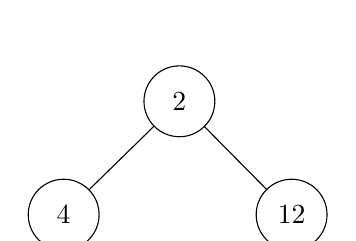
\begin{tikzpicture}[scale=0.15]
\tikzstyle{every node}+=[inner sep=0pt]
\draw [black] (34.5,-8.7) circle (3);
\draw (34.5,-8.7) node {$2$};
\draw [black] (24.7,-18.3) circle (3);
\draw (24.7,-18.3) node {$4$};
\draw [black] (44,-18.3) circle (3);
\draw (44,-18.3) node {$12$};
\draw [black] (32.36,-10.8) -- (26.84,-16.2);
\draw [black] (36.61,-10.83) -- (41.89,-16.17);
\end{tikzpicture}
\end{center}
Schritt 3: 3. Array-Element wird in Heap eingefügt. Heap-Eigenschaft erfüllt, kein Austausch.\\

\begin{center}
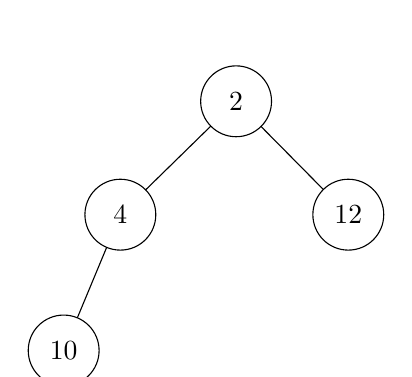
\begin{tikzpicture}[scale=0.15]
\tikzstyle{every node}+=[inner sep=0pt]
\draw [black] (34.5,-8.7) circle (3);
\draw (34.5,-8.7) node {$2$};
\draw [black] (24.7,-18.3) circle (3);
\draw (24.7,-18.3) node {$4$};
\draw [black] (44,-18.3) circle (3);
\draw (44,-18.3) node {$12$};
\draw [black] (19.9,-29.8) circle (3);
\draw (19.9,-29.8) node {$10$};
\draw [black] (32.36,-10.8) -- (26.84,-16.2);
\draw [black] (36.61,-10.83) -- (41.89,-16.17);
\draw [black] (23.54,-21.07) -- (21.06,-27.03);
\end{tikzpicture}
\end{center}
Schritt 4: 4. Array-Element in Heap einfügen. Heap-Eigenschaft erfüllt, kein Austausch.\\

\begin{center}
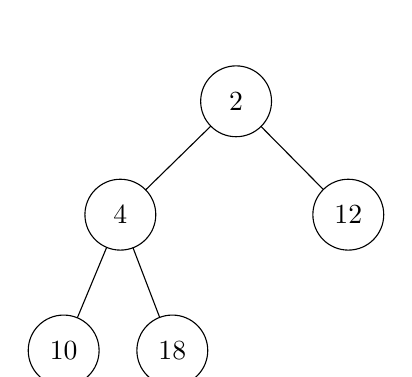
\begin{tikzpicture}[scale=0.15]
\tikzstyle{every node}+=[inner sep=0pt]
\draw [black] (34.5,-8.7) circle (3);
\draw (34.5,-8.7) node {$2$};
\draw [black] (24.7,-18.3) circle (3);
\draw (24.7,-18.3) node {$4$};
\draw [black] (44,-18.3) circle (3);
\draw (44,-18.3) node {$12$};
\draw [black] (19.9,-29.8) circle (3);
\draw (19.9,-29.8) node {$10$};
\draw [black] (29.1,-29.8) circle (3);
\draw (29.1,-29.8) node {$18$};
\draw [black] (32.36,-10.8) -- (26.84,-16.2);
\draw [black] (36.61,-10.83) -- (41.89,-16.17);
\draw [black] (23.54,-21.07) -- (21.06,-27.03);
\draw [black] (25.77,-21.1) -- (28.03,-27);
\end{tikzpicture}
\end{center}
Schritt 5: 5. Array-Element wird in Heap eingefügt. Heap-Eigenschaft erfüllt, kein Austausch.\\

\begin{center}
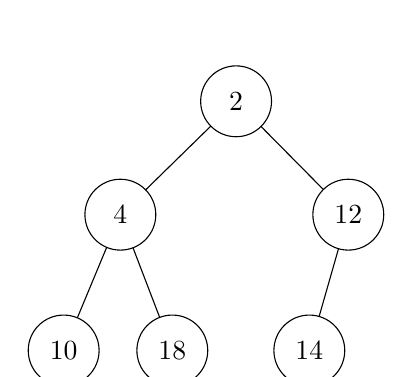
\begin{tikzpicture}[scale=0.15]
\tikzstyle{every node}+=[inner sep=0pt]
\draw [black] (34.5,-8.7) circle (3);
\draw (34.5,-8.7) node {$2$};
\draw [black] (24.7,-18.3) circle (3);
\draw (24.7,-18.3) node {$4$};
\draw [black] (44,-18.3) circle (3);
\draw (44,-18.3) node {$12$};
\draw [black] (19.9,-29.8) circle (3);
\draw (19.9,-29.8) node {$10$};
\draw [black] (29.1,-29.8) circle (3);
\draw (29.1,-29.8) node {$18$};
\draw [black] (40.7,-29.8) circle (3);
\draw (40.7,-29.8) node {$14$};
\draw [black] (32.36,-10.8) -- (26.84,-16.2);
\draw [black] (36.61,-10.83) -- (41.89,-16.17);
\draw [black] (23.54,-21.07) -- (21.06,-27.03);
\draw [black] (25.77,-21.1) -- (28.03,-27);
\draw [black] (43.17,-21.18) -- (41.53,-26.92);
\end{tikzpicture}
\end{center}
Schritt 6: 6. Array-Element wird eingefügt. Heap-Eigenschaft erfüllt, kein Austausch.\\

\begin{center}
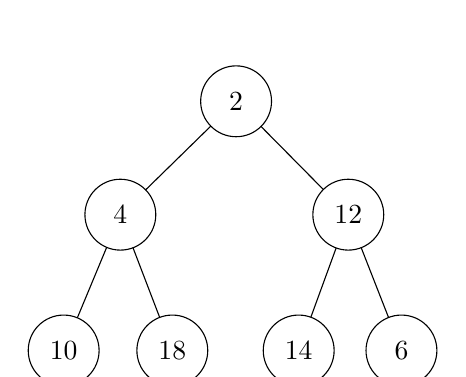
\begin{tikzpicture}[scale=0.15]
\tikzstyle{every node}+=[inner sep=0pt]
\draw [black] (34.5,-8.7) circle (3);
\draw (34.5,-8.7) node {$2$};
\draw [black] (24.7,-18.3) circle (3);
\draw (24.7,-18.3) node {$4$};
\draw [black] (44,-18.3) circle (3);
\draw (44,-18.3) node {$12$};
\draw [black] (19.9,-29.8) circle (3);
\draw (19.9,-29.8) node {$10$};
\draw [black] (29.1,-29.8) circle (3);
\draw (29.1,-29.8) node {$18$};
\draw [black] (39.8,-29.8) circle (3);
\draw (39.8,-29.8) node {$14$};
\draw [black] (48.5,-29.8) circle (3);
\draw (48.5,-29.8) node {$6$};
\draw [black] (32.36,-10.8) -- (26.84,-16.2);
\draw [black] (36.61,-10.83) -- (41.89,-16.17);
\draw [black] (23.54,-21.07) -- (21.06,-27.03);
\draw [black] (25.77,-21.1) -- (28.03,-27);
\draw [black] (42.97,-21.12) -- (40.83,-26.98);
\draw [black] (45.09,-21.09) -- (47.41,-27.01);
\end{tikzpicture}
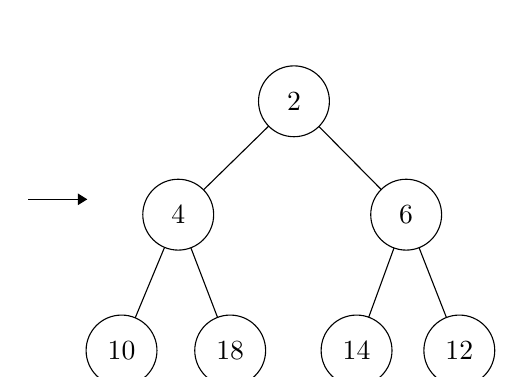
\begin{tikzpicture}[scale=0.15]
\tikzstyle{every node}+=[inner sep=0pt]
\draw [black] (12.00,-17.00) -- (17.00,-17.00);
\fill [black] (17.00,-17.00) -- (16.2,-16.5) -- (16.2,-17.5);
\draw [black] (34.5,-8.7) circle (3);
\draw (34.5,-8.7) node {$2$};
\draw [black] (24.7,-18.3) circle (3);
\draw (24.7,-18.3) node {$4$};
\draw [black] (44,-18.3) circle (3);
\draw (44,-18.3) node {$6$};
\draw [black] (19.9,-29.8) circle (3);
\draw (19.9,-29.8) node {$10$};
\draw [black] (29.1,-29.8) circle (3);
\draw (29.1,-29.8) node {$18$};
\draw [black] (39.8,-29.8) circle (3);
\draw (39.8,-29.8) node {$14$};
\draw [black] (48.5,-29.8) circle (3);
\draw (48.5,-29.8) node {$12$};
\draw [black] (32.36,-10.8) -- (26.84,-16.2);
\draw [black] (36.61,-10.83) -- (41.89,-16.17);
\draw [black] (23.54,-21.07) -- (21.06,-27.03);
\draw [black] (25.77,-21.1) -- (28.03,-27);
\draw [black] (42.97,-21.12) -- (40.83,-26.98);
\draw [black] (45.09,-21.09) -- (47.41,-27.01);
\end{tikzpicture}
\end{center}
Schritt 7: 7. Array-Element wird in Heap eingefügt und Heap-Eigenschaft geprüft und hergestellt.\\

\begin{center}
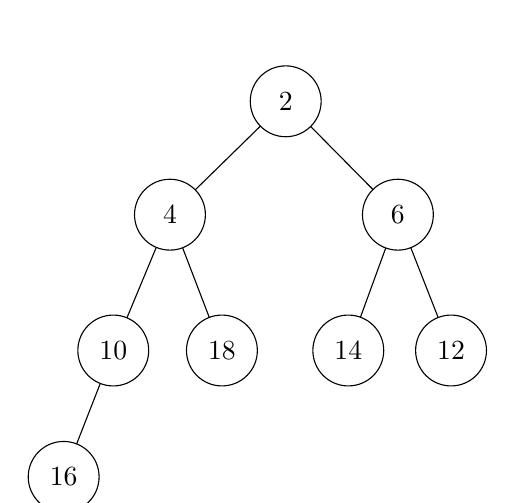
\begin{tikzpicture}[scale=0.15]
\tikzstyle{every node}+=[inner sep=0pt]
\draw [black] (34.5,-8.7) circle (3);
\draw (34.5,-8.7) node {$2$};
\draw [black] (24.7,-18.3) circle (3);
\draw (24.7,-18.3) node {$4$};
\draw [black] (44,-18.3) circle (3);
\draw (44,-18.3) node {$6$};
\draw [black] (19.9,-29.8) circle (3);
\draw (19.9,-29.8) node {$10$};
\draw [black] (29.1,-29.8) circle (3);
\draw (29.1,-29.8) node {$18$};
\draw [black] (39.8,-29.8) circle (3);
\draw (39.8,-29.8) node {$14$};
\draw [black] (48.5,-29.8) circle (3);
\draw (48.5,-29.8) node {$12$};
\draw [black] (15.7,-40.5) circle (3);
\draw (15.7,-40.5) node {$16$};
\draw [black] (32.36,-10.8) -- (26.84,-16.2);
\draw [black] (36.61,-10.83) -- (41.89,-16.17);
\draw [black] (23.54,-21.07) -- (21.06,-27.03);
\draw [black] (25.77,-21.1) -- (28.03,-27);
\draw [black] (42.97,-21.12) -- (40.83,-26.98);
\draw [black] (45.09,-21.09) -- (47.41,-27.01);
\draw [black] (18.8,-32.59) -- (16.8,-37.71);
\end{tikzpicture}
\end{center}
Schritt 8: 8. Array-Element wird in Heap eingefügt. Heap-Eigenschaft erfüllt, kein Austausch.\\

\begin{center}
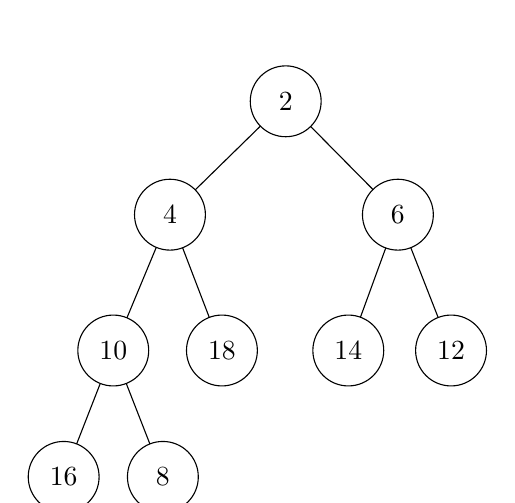
\begin{tikzpicture}[scale=0.15]
\tikzstyle{every node}+=[inner sep=0pt]
\draw [black] (34.5,-8.7) circle (3);
\draw (34.5,-8.7) node {$2$};
\draw [black] (24.7,-18.3) circle (3);
\draw (24.7,-18.3) node {$4$};
\draw [black] (44,-18.3) circle (3);
\draw (44,-18.3) node {$6$};
\draw [black] (19.9,-29.8) circle (3);
\draw (19.9,-29.8) node {$10$};
\draw [black] (29.1,-29.8) circle (3);
\draw (29.1,-29.8) node {$18$};
\draw [black] (39.8,-29.8) circle (3);
\draw (39.8,-29.8) node {$14$};
\draw [black] (48.5,-29.8) circle (3);
\draw (48.5,-29.8) node {$12$};
\draw [black] (15.7,-40.5) circle (3);
\draw (15.7,-40.5) node {$16$};
\draw [black] (24.1,-40.5) circle (3);
\draw (24.1,-40.5) node {$8$};
\draw [black] (32.36,-10.8) -- (26.84,-16.2);
\draw [black] (36.61,-10.83) -- (41.89,-16.17);
\draw [black] (23.54,-21.07) -- (21.06,-27.03);
\draw [black] (25.77,-21.1) -- (28.03,-27);
\draw [black] (42.97,-21.12) -- (40.83,-26.98);
\draw [black] (45.09,-21.09) -- (47.41,-27.01);
\draw [black] (18.8,-32.59) -- (16.8,-37.71);
\draw [black] (21,-32.59) -- (23,-37.71);
\end{tikzpicture}
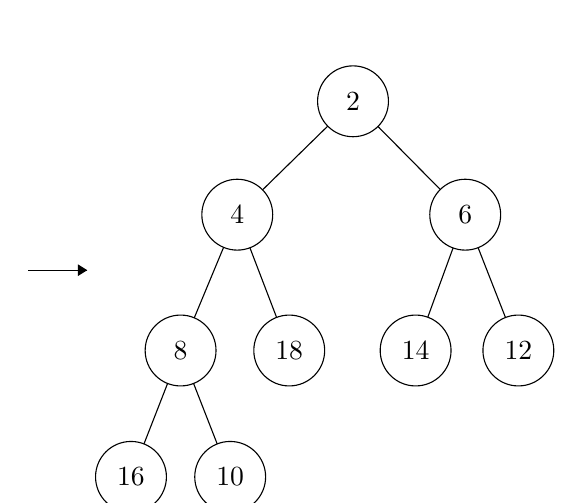
\begin{tikzpicture}[scale=0.15]
\tikzstyle{every node}+=[inner sep=0pt]
\draw [black] (7.00,-23.00) -- (12.00,-23.00);
\fill [black] (12.00,-23.00) -- (11.2,-22.5) -- (11.2,-23.5);
\draw [black] (34.5,-8.7) circle (3);
\draw (34.5,-8.7) node {$2$};
\draw [black] (24.7,-18.3) circle (3);
\draw (24.7,-18.3) node {$4$};
\draw [black] (44,-18.3) circle (3);
\draw (44,-18.3) node {$6$};
\draw [black] (19.9,-29.8) circle (3);
\draw (19.9,-29.8) node {$8$};
\draw [black] (29.1,-29.8) circle (3);
\draw (29.1,-29.8) node {$18$};
\draw [black] (39.8,-29.8) circle (3);
\draw (39.8,-29.8) node {$14$};
\draw [black] (48.5,-29.8) circle (3);
\draw (48.5,-29.8) node {$12$};
\draw [black] (15.7,-40.5) circle (3);
\draw (15.7,-40.5) node {$16$};
\draw [black] (24.1,-40.5) circle (3);
\draw (24.1,-40.5) node {$10$};
\draw [black] (32.36,-10.8) -- (26.84,-16.2);
\draw [black] (36.61,-10.83) -- (41.89,-16.17);
\draw [black] (23.54,-21.07) -- (21.06,-27.03);
\draw [black] (25.77,-21.1) -- (28.03,-27);
\draw [black] (42.97,-21.12) -- (40.83,-26.98);
\draw [black] (45.09,-21.09) -- (47.41,-27.01);
\draw [black] (18.8,-32.59) -- (16.8,-37.71);
\draw [black] (21,-32.59) -- (23,-37.71);
\end{tikzpicture}
\end{center}
Schritt 9: 9. und letztes Array-Element wird in Heap einfügen und Heap-Eigenschaft wird geprüft und hergestellt. Min-Heap ist vollständig erstellt.

\paragraph{b)}
Wie sieht der Heap aus, wenn Sie eine \textsc{ExtractMin} Operation ausgeführt und dann die Heapeigenschaft wieder hergestellt haben? \\

Nach ExtractMin:
\begin{center}
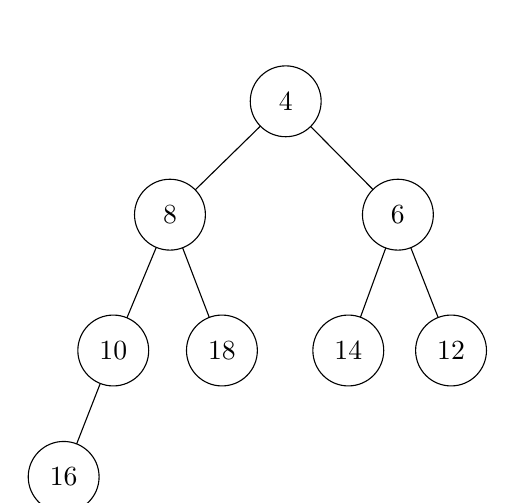
\begin{tikzpicture}[scale=0.15]
\tikzstyle{every node}+=[inner sep=0pt]
\draw [black] (34.5,-8.7) circle (3);
\draw (34.5,-8.7) node {$4$};
\draw [black] (24.7,-18.3) circle (3);
\draw (24.7,-18.3) node {$8$};
\draw [black] (44,-18.3) circle (3);
\draw (44,-18.3) node {$6$};
\draw [black] (19.9,-29.8) circle (3);
\draw (19.9,-29.8) node {$10$};
\draw [black] (29.1,-29.8) circle (3);
\draw (29.1,-29.8) node {$18$};
\draw [black] (39.8,-29.8) circle (3);
\draw (39.8,-29.8) node {$14$};
\draw [black] (48.5,-29.8) circle (3);
\draw (48.5,-29.8) node {$12$};
\draw [black] (15.7,-40.5) circle (3);
\draw (15.7,-40.5) node {$16$};
\draw [black] (32.36,-10.8) -- (26.84,-16.2);
\draw [black] (36.61,-10.83) -- (41.89,-16.17);
\draw [black] (23.54,-21.07) -- (21.06,-27.03);
\draw [black] (25.77,-21.1) -- (28.03,-27);
\draw [black] (42.97,-21.12) -- (40.83,-26.98);
\draw [black] (45.09,-21.09) -- (47.41,-27.01);
\draw [black] (18.8,-32.59) -- (16.8,-37.71);
\end{tikzpicture}
\end{center}

Durch Extractmin wird die Wurzel entfernt, da Wurzel das kleinste Element ist.\\
Dann wird 10 zur Wurzel und sinkt nach unten.\\
Dabei wird erst 10  mit 4 getauscht und anschließend 10 mit 8 vertauscht.\\

\paragraph{c)}
Fügen Sie das neue Element $3$ zu dem Heap (aus b) hinzu. \\

\begin{center}
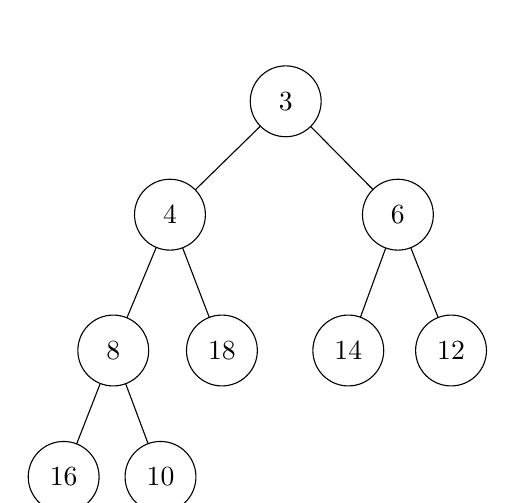
\begin{tikzpicture}[scale=0.15]
\tikzstyle{every node}+=[inner sep=0pt]
\draw [black] (34.5,-8.7) circle (3);
\draw (34.5,-8.7) node {$3$};
\draw [black] (24.7,-18.3) circle (3);
\draw (24.7,-18.3) node {$4$};
\draw [black] (44,-18.3) circle (3);
\draw (44,-18.3) node {$6$};
\draw [black] (19.9,-29.8) circle (3);
\draw (19.9,-29.8) node {$8$};
\draw [black] (29.1,-29.8) circle (3);
\draw (29.1,-29.8) node {$18$};
\draw [black] (39.8,-29.8) circle (3);
\draw (39.8,-29.8) node {$14$};
\draw [black] (48.5,-29.8) circle (3);
\draw (48.5,-29.8) node {$12$};
\draw [black] (15.7,-40.5) circle (3);
\draw (15.7,-40.5) node {$16$};
\draw [black] (23.9,-40.5) circle (3);
\draw (23.9,-40.5) node {$10$};
\draw [black] (32.36,-10.8) -- (26.84,-16.2);
\draw [black] (36.61,-10.83) -- (41.89,-16.17);
\draw [black] (23.54,-21.07) -- (21.06,-27.03);
\draw [black] (25.77,-21.1) -- (28.03,-27);
\draw [black] (42.97,-21.12) -- (40.83,-26.98);
\draw [black] (45.09,-21.09) -- (47.41,-27.01);
\draw [black] (18.8,-32.59) -- (16.8,-37.71);
\draw [black] (20.95,-32.61) -- (22.85,-37.69);
\end{tikzpicture}
\end{center}
Das Element 3 wird am Ende des Arrays angehängt und anschließend die Heapeigenschaft getestet.\\
3 steigt dabei nach dem Vergleich mit der 10, 8 und 4 bis zur Wurzel auf.\\

\paragraph{d)}
Analysieren Sie in $\mathcal{O}$-Notation die Laufzeit der Methode \textsc{ExtractMax}, die das maximale Element aus einem Min-Heap $S$ der Größe $n$ löscht. \\

ExtractMax benötigt n - 1 Schritte, um alle Blätter des Heaps zu finden und dann noch einmal maximal $2^{Hoehe(H)}+1$ Schritte für den Vergleich der Blätter, das Finden und das Löschen des Maximums.\\
Weil die Höhe des Heaps bei jeder nächsten Zweierpotenz um 1 steigt, haben wir $Hoehe(H) = \lfloor \log_2 n \rfloor$, also die Laufzeit $T(n) = n-1 + 2^{Hoehe(H)}+1 \leq n+2^{\log_2 n} = n + n = 2n \Rightarrow \mathcal{O}(n)$.

%----------------------------------------------------------------------------
\section{Eine Erweiterung von Heapsort}
In der Vorlesung haben Sie das Sortierverfahren Heapsort kennengelernt. Wir betrachten nun eine Erweiterung dieses Verfahrens, das sogenannte \emph{$k$-Heapsort}. Dabei ist $k\ge2$ eine natürliche Zahl. Bei diesem Verfahren benutzt man statt einem Binärbaum einen $k$-nären Baum, bei dem jeder Knoten höchstens $k$ Kinder hat. Deshalb heißt der korrespondierende Heap $k$-Heap. 

\paragraph{a)}
Wie kann man einen $k$-Heap als ein Array repräsentieren? Wie effizient ist es, die Kinder bzw. den Elternknoten eines gegebenen Knoten zu finden? \\

Array A$[a_0 ..... a_n]$

Root: $a_0$\\
1st Level: $a_1 ..... a_{2+k}$ \\
2nd Level: $a_{1+k} ...... a_{2+k+k^2}$\\
.\\
.\\
.\\
nth Level: $a_{1+ \sum_{i=1}^{n-1} {k^i}} ... a_{\sum_{i=1}^{n} {k^i}}$\\

Parent nodes of i: $\lfloor{(i-1)/k}\rfloor$\\
Child nodes j of i: $i*k +j$ ($1\leq j \leq k$)\\


\paragraph{b)} Geben Sie die Höhe eines $k$-Heaps an, wenn dieser $n$ Elemente enthält. \\

h = $\lceil log_k((n * k) - (n + 1))\rceil - 1$

\paragraph{c)} 
Geben Sie Pseudocode für effiziente Implementierungen der Methoden \texttt{Insert} und \texttt{ExtractMin} an. Analysieren Sie die Komplexität der beiden Methoden in Abhängigkeit von $n$ und $k$. \\

A = Array, X = Element, I = Index, k

\begin{lstlisting}
Insert(A, X, k) {
    Increase length of A by 1
    Insert X at A[length(A)]
    HeapUp(A, length(A) - 1, k)
}

HeapUp(Array A, i, k) {
    
    while (i not root){
    
      if (array[i] > array[parent-position] {
          Swap A[i] and A[parent-position]
          i = parent
          parent = (i-1)/k
      }
      else 
      	break
	}
}

\end{lstlisting}
Complexity:\\
Because we need a comparison for each tree-level: Insert() $\in \mathcal{O}(log_k((n*k) - (n+1))$\\
	
\begin{lstlisting}
ExtractMin(Array A)
{
	Extract root
    Set length(A)-1 (last element) as new root
    Shorten array by 1
    HeapDown(A, root)
}

HeapDown(array A, node n)
{
	for (n not leaf){
    	compare n to its childs 1 - k step by step
        	if(n < child){
            	swap (n, child)                
            }
         HeapDown(A, child)
             
    }
}

\end{lstlisting}
Complexity:\\
We need k comparisons on every level, thats why extractMin() $\in \mathcal{O}(3 log_k(n*k - n) $.\\

%----------------------------------------------------------------------------
\section{Zwei-Drittel-Sortieren}
Eine alternative Methode, um ein Array $A$ der Länge $n$ zu sortieren, ist die Folgende:

\begin{algorithm}[H]
	\If{$A[left] > A[right]$} {
		exchange $A[left]$ and $A[right]$ \;
	}
	\If{$left + 1 \ge right$} {
		\Return \;
	}
	$k \longleftarrow \left\lfloor \frac{right - left + 1}3 \right\rfloor$ \;
	\texttt{ZweiDrittelSortieren}($A$, $left$, $right-k$)\;
	\texttt{ZweiDrittelSortieren}($A$, $left+k$, $right$)\;
	\texttt{ZweiDrittelSortieren}($A$, $left$, $right-k$)\;
 \caption{\texttt{ZweiDrittelSortieren}($A$, $left$, $right$)}
 \label{algo:ZweiDrittelSortieren}
\end{algorithm}

\paragraph{a)}
Argumentieren Sie, dass \texttt{ZweiDrittelSortieren}($A$, $1$, $n$) das Array $A[1..n]$ korrekt sortiert. \\

Argumentation, dass Zwei-Drittel-Sortieren korrekt ist, mithilfe von Induktion über die Länge des sortierten Teilarrays k: ($right-left+1$).\\
Für Länge 1 ist das Array immer sortiert, für Länge 2 muss einmal verglichen und gegebenenfalls ausgetauscht werden.\\
\\
Für Längen > 2 sei $k = (right-left+1)/3$.\\
Betrachte nun die k größten Elemente des Arrays von left bis right.\\
$m \leq k$ Elemente sind in den ersten zwei Dritteln des Arrays und gleichzeitig sind $m$ die größten Elemente dieses Teilarrays.\\
Nach der ersten Rekursion, die das Teilarray korrekt sortiert hat (Induktionsvoraussetzung korrekt), befinden sich diese $m$ Elemente im Teilarray A[$right-k-m+1$]...A[$right-k$] mit der Eigenschaft $right-k-m+1 \geq left+k$.\\
\\
Das mittlere Drittel besteht aus mindestens k Elementen und die k größten Elemente befinden sich zwischen $left + k$ und $right$, also sind diese auch nach dem zweiten Aufruf korrekt sortiert.\\
Im letzten Drittel des Arrays die (übrigens) $\leq$ k größten Elemente, welche im letzten rekursiven Aufruf sortiert werden.

\paragraph{b)}
Analysieren Sie die Laufzeit von \texttt{ZweiDrittelSortieren} im worst-case. Geben Sie Ihre Angaben in $\mathcal{O}$-Notation an. \\

Worst-Case: In jedem Rekursionsschritt werden zwei Elemente ($left$, $right$ des jeweiligen Teilarrays) getauscht werden und anschließend weiter gedrittelt, daher $T(n) = 3*T(\frac{n}{3})+2$.\\
\\
Mastertheorem:\\
$a = 3,$ $b= 3,$ $f(n) = 2*n^0$\\
$f(n) = 2*n^{1-1} = 2*n^{\log_3(3)-1} \in \mathcal{O}(n^{\log_3(3)-\epsilon})$ wobei $\epsilon = 1$\\
$\Rightarrow T(n) \in \Theta(n^{\log_3(3)}) \in \Theta(n^1) \in \Theta(n)$

\paragraph{c)}
Ist Zwei-Drittel-Sortieren im worst-case effizienter als Insertsort, Minimumsuche+Austauschen, Quicksort oder Heapsort? Alle Antworten sollten jeweils ausreichend begründet werden. \\

Insertion Sort Worst-Case Laufzeit:\\
$T(n) = \frac{n^2+n}{2} = \mathcal{O}(n^2)$, zwei-Drittel-Sortieren ist also deutlich schneller.\\
Minimumsuche + Austausch hat eine Worst-Case Laufzeit von $T(n) = \frac{n^2+n}{2} = \mathcal{O}(n^2)$, zwei-Drittel-Sortieren ist also deutlich schneller.\\
Quicksort hat die Worst-Case Laufzeit $\mathcal{O}(n^2)$, zwei-Drittel-Sortieren ist also deutlich schneller.\\
Heapsort hat die Worst-Case Laufzeit $\mathcal{O}(n \log n)$, zwei-Drittel-Sortieren ist also etwas schneller.

%----------------------------------------------------------------------------

\end{document}